\newpage
\section{Eigenständigkeitserklärung}
% Hiermit erkläre ich, Lukas Wessel, dass ich die vorliegende Projektarbeit mit dem Titel \glqq Neugestaltung von \textit{Schüler Online}: Eine Beobachtungs- und Interviewstudie zur Identifikation von Problemstellen und Nutzerbedürfnissen, um die Effektivität sowie die Zufriedenstellung des Schulpersonals beim Erfüllen von Kernaufgaben der Webanwendung zu optimieren\grqq{} selbstständig und ohne fremde Hilfe verfasst habe. Alle verwendeten Quellen und Hilfsmittel sind im Literaturverzeichnis vollständig und korrekt angegeben.

% Sämtliche Textstellen, die wörtlich oder sinngemäß aus veröffentlichten oder nicht veröffentlichten Schriften entnommen wurden, sind als solche kenntlich gemacht. Die Arbeit hat in gleicher oder ähnlicher Form noch keiner Prüfungsbehörde vorgelegen.

% Ich bin mir bewusst, dass eine falsche Erklärung rechtliche Konsequenzen haben wird.
% \\\\

% Ort, Datum: 
% \\\\

% Unterschrift: 
\begin{figure}[H]
    \centering
    \begin{adjustbox}{width=\linewidth, center}
        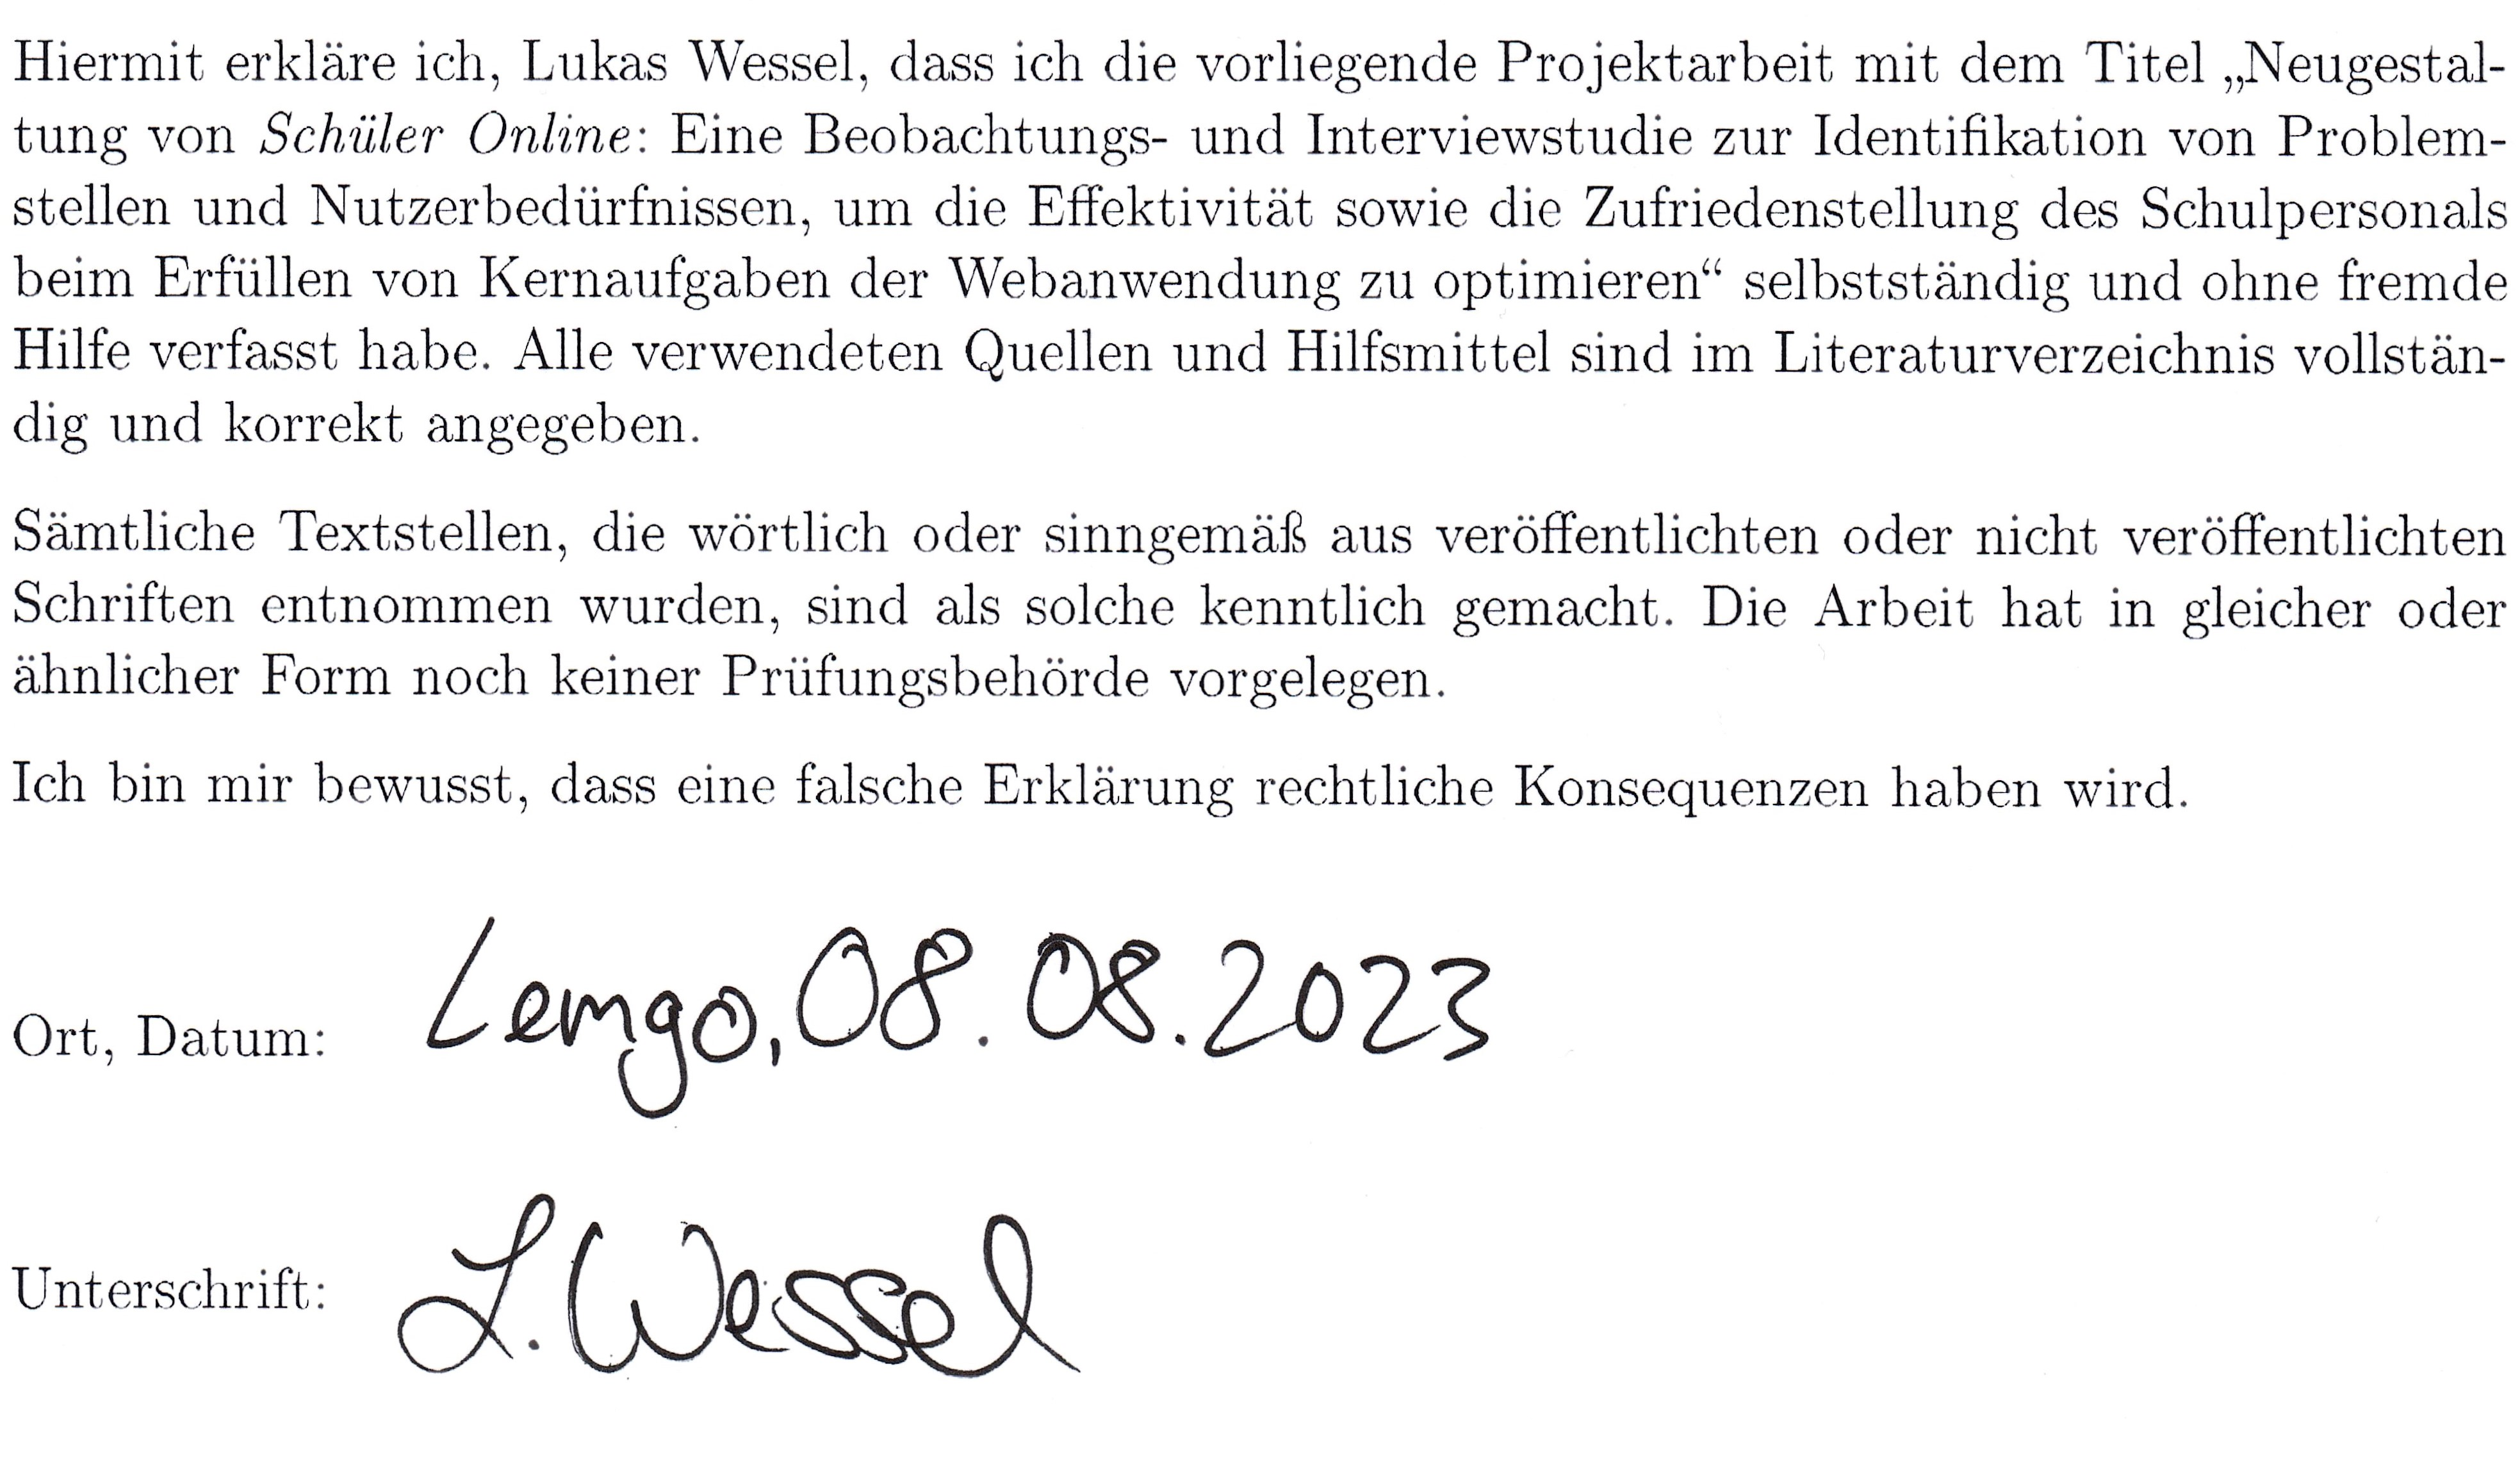
\includegraphics{eigenstaendigkeitserklaerung}
    \end{adjustbox}
\end{figure}

